\documentclass[12pt, a4paper]{article}
\usepackage[utf8]{inputenc}
\usepackage{graphicx}
\usepackage{amsmath}
\graphicspath{{images/}}
 
 
\title{Project Proposal}
\author{Edward Gill \thanks{To Me...I am Unstoppable}}
\date{February 2019}

\begin{document}
\maketitle

\begin{abstract}
This is the start of a journey that is likely to be frought with dangers, both hidden and seen, stay strong my son, for you will prevail. Even in the deepest of dark, remain steady, unperturbed and you shall exit with glory intact.
\end{abstract}
\tableofcontents
\clearpage
This proposal will outline how and why I am undertaking my main topic, this should be very fun mutha fucker

The watery finger of God 
\begin{figure}[h]
    \centering
% below is where you put the acutal image name in the directory
    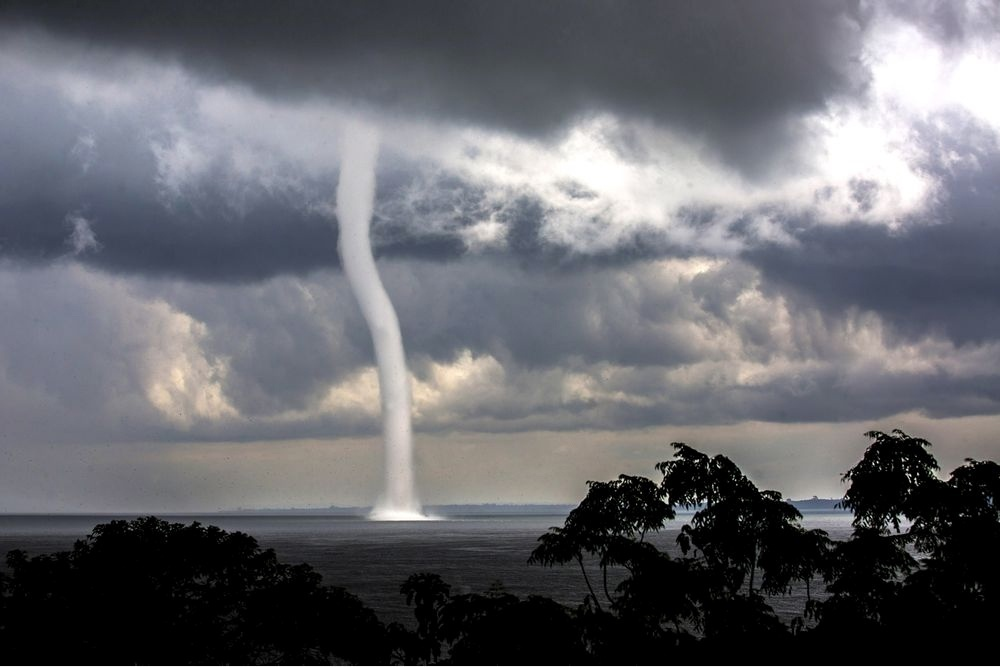
\includegraphics[width=0.25\textwidth]{uganda}
    \caption{Watery Finger}
 %  below is only a naming convention, above is the real deal
    \label{fig:ass}
\end{figure}
 
As you can see in the figure \ref{fig:ass}, the 
function grows near 0. Also, in the page \pageref{fig:ass} 
is the same example.

% this moves us to a new page...
\clearpage

\begin{itemize}
  \item Outline your goals here
  \item Make Love Not War
\end{itemize}

\clearpage

\section{introduction}

In physics, the mass-energy equivalence is stated 
by the equation $E=mc^2$, discovered in 1905 by Albert Einstein.
\begin{math}
x^2 = X^{sex}+ exp*52
\end{math}
But the alas, the secret to life as we know it is found below
You are the product of your environment
\begin{equation}
You = Env^2
\end{equation}
\subsection{First Section}

$$T^{i_1 i_2 \dots i_p}_{j_1 j_2 \dots j_q} = T(x^{i_1},\dots,x^{i_p},e_{j_1},\dots,e_{j_q})$$
 
We write integrals using $\int$ and fractions using $\frac{a}{b}$. Limits are placed on integrals using superscripts and subscripts:
 
$$\int_0^1 \frac{1}{e^x} =  \frac{e-1}{e}$$
 
Lower case Greek letters are written as $\omega$ $\delta$ etc. while upper case Greek letters are written as $\Omega$ $\Delta$.
 
Mathematical operators are prefixed with a backslash as $\sin(\beta)$, $\cos(\alpha)$, $\log(x)$ etc.


\end{document}